\subsection{Class Diagram}

\begin{figure}[H]
    \centering
    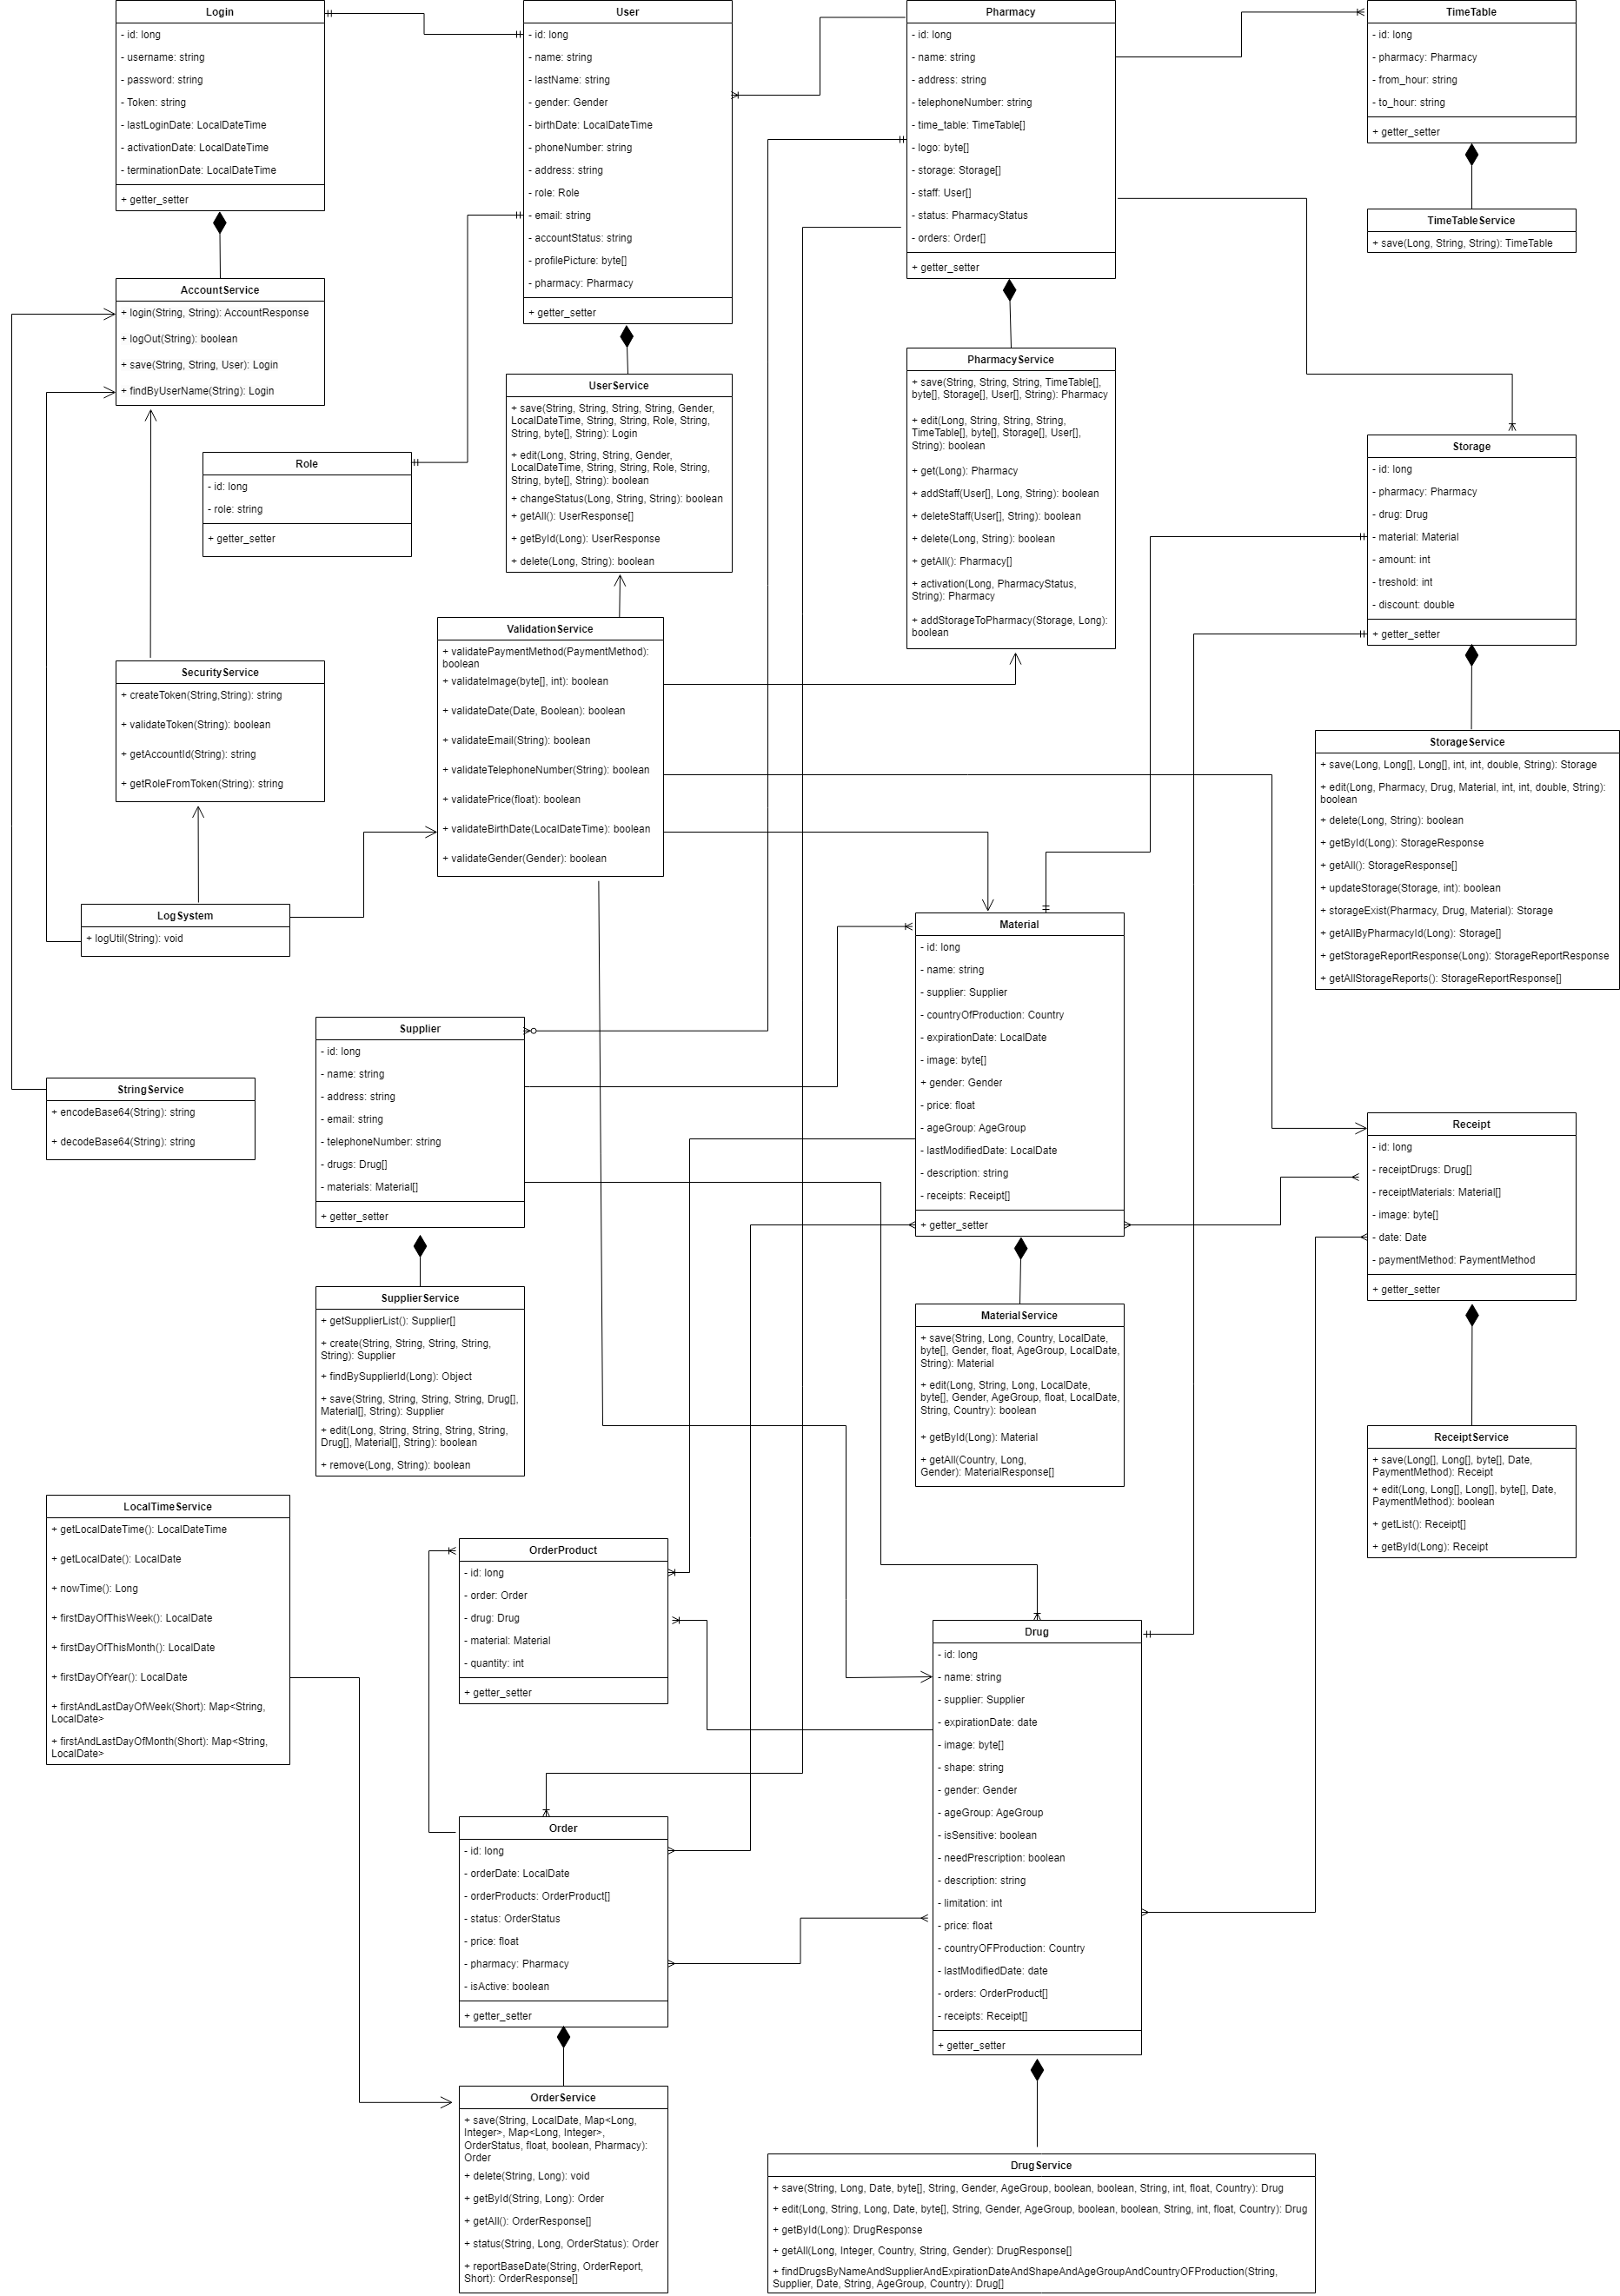
\includegraphics[width=0.75\textwidth]{sections/BLL/class_diagram.png}
    \caption{Class Diagram}
    \label{fig:my_CD}
\end{figure}
%Describe here the class diagram of your project

The class diagram (Figure~\ref{fig:my_CD}) consists of several classes that represent the entities and services in the system. Here's a brief overview of each class and its purpose:

\begin{itemize}
\item Login: This class represents a user account in the system. It contains the username and password fields, which are used for authentication. The Account class is used by the service to handle login, logout, and account creation.

\item User: This class represents a user in the system. It contains fields such as name, username, password, and email, as well as additional fields such as gender, birth date, and address. The User class is used by the UserService to handle user management, such as adding, editing, and deleting user accounts.
\item Pharmacy: This class represents a pharmacy in the system. It contains fields such as name, address, and phone number, as well as a list of staff members, storage items, and timetables. The Pharmacy class is used by the PharmacyService to handle pharmacy management, such as adding, editing, and deleting pharmacy accounts.

\item TimeTable: This class represents a weekly timetable that defines the working hours of a pharmacy. It contains the fromHour and toHour fields, which represent the start and end times of a workday. The TimeTable class is used by the Pharmacy class to define the working hours of a pharmacy.

\item Drug: This class represents a  drug that can be stored in a pharmacy. It contains fields such as name, supplier, expiration date, price, and additional fields such as age group and country of production. The Drug class is used by the DrugService to handle drug management, such as adding, editing, and deleting materials/drugs.

\item Material: The Material class is a class that shares similarities with a drug class. It has various attributes such as name, supplier, expiration date, and price, as well as extra attributes like the age group and country where it was produced. The MaterialService utilizes this class to perform tasks related to material management including adding, modifying, and removing materials.

\item Supplier: This class represents a supplier of materials/drugs. It contains fields such as name, address, email, and telephone number. The Supplier class is used by the Material/Drug class to specify the supplier of a material/drug.

\item Storage: This class represents a storage item in a pharmacy, which associates a material/drug with a quantity. It contains fields such as pharmacy, drug, and quantity. The Storage class is used by the Pharmacy class to manage the inventory of a pharmacy.

\item Order: This class represents an order placed by a user. It contains fields such as date, total cost, user, and a list of order items. The Order class represents a customer's order, which can be fulfilled by a pharmacy.

\item Role: The Role class represents a role in the system. It contains fields such as id and role, which are used to uniquely identify a role and its name, respectively.

\item LogSystem: This interface represents a system for logging messages. It contains a single method, logUtil, which takes a message as input and logs it into the system. 

\item OrderProduct: The OrderProduct class represents an individual product within an order. It contains fields such as the product's unique identifier (id), the order it belongs to (order), the drug or material being ordered (drug or material), and the quantity being ordered (quantity). This class is used by the Order class to specify the products included in an order.

\item StringService: StringService is an interface that provides two methods for encoding and decoding strings using Base64. The encodeBase64() method takes an input string and returns its Base64-encoded equivalent. The decodeBase64() method takes a Base64-encoded string and returns its decoded value. 

\item SecurityService: This interface represents a security service in the system. It provides methods for creating and validating tokens, as well as retrieving information from tokens. The create token method takes in an accountId and role and generates a unique token that can be used for authentication purposes. The validateToken method checks if a token is valid or not. The getAccountId method extracts the accountId from a given token, while the getRoleFromToken method extracts the role from a given token. These methods are used by other services to ensure secure access to sensitive information and operations in the system.

\item LocalTimeService: LocalTimeService is an interface that provides access to methods for working with local dates and times. It has three methods: getLocalDateTime(), which returns the current date and time in the system's default time zone; getLocalDate(), which returns the current date in the system's default time zone; and nowTime(), which returns the current time in milliseconds since the Unix epoch (January 1, 1970, 00:00:00 GMT).

\item AccountService: AccountService is an interface that represents the functionality of a service responsible for managing user accounts. It provides methods for login, logout, and creating a new user account. The login method takes in the username and password of a user and returns an AccountResponse object, which contains information about the user account, including a token for future authentication. The logout method takes in a token and logs out the user associated with that token. The save method is used to create a new user account and takes in the username, password, and user information. The findByUserName method is used to find a user account based on the username.

\item ValidationService: ValidationService is an interface that defines methods to validate certain types of data used in the system. It contains methods to validate payment methods, images, dates, email addresses, telephone numbers, prices, birth dates, and gender. The methods take input parameters of the data to be validated and return a Boolean value indicating whether the data is valid or not. By providing a centralized place for data validation, the validation service helps to ensure consistency and accuracy throughout the system.

\end{itemize}